\section{Einführung}
Der Vier-Farben-Satz ist eines der am simpelsten zu erklärenden Probleme. Er besagt, dass man jede Karte mit vier Farben oder weniger einfärben kann, ohne dass sich dabei zwei Flächen gleicher Farbe berühren. Es ist insofern einfach, dass man den Vier-Farben-Satz einem acht-jährigem Kind schildern könnte und ihm die Grundaussage klar wäre. Es ist relativ einfach eine Karte zu finden, welche mehr als drei Farben benötigt, auch ist es relativ einfach einen Weg zu finden um eine Karte mit fünf einzufärben. Das wahrscheinlich Bekannteste am Vier-Farben-Satz ist nicht der Fakt, dass man jede Karte mit nur vier Farben einfärben kann, sondern dass das Problem im Verhältnis zur Komplexität des Beweises so leicht zu erklären ist.

\begin{center}
    \begin{figure}[h]
        \centering
            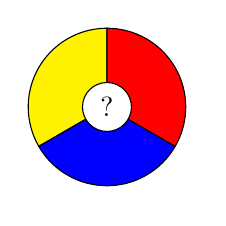
\begin{tikzpicture}
            \draw[fill=yellow] (0,0) -- (90:1cm) arc (90:90+120:1cm) -- (0,0);
            \draw[fill=blue] (0,0) -- (90+120:1cm) arc (90+120:90+120+120:1cm) -- (0,0);
            \draw[fill=red] (0,0) -- (90+120+120:1cm) arc (90+120+120:90+120+120+120:1cm) -- (0,0);
            \node[circle,draw=black,fill=white] (middle) at (0,0) {?};
            \end{tikzpicture}
        \caption{Beispiel für vier Farben}
        \label{fig:my_label}
    \end{figure}
    
    
\end{center}